
% page 4
\frame{
    \frametitle{6.4.1 線形回帰モデル再び}
    3章でやった線形回帰モデルを用いる。

    \begin{align}
        y(\mathbf{x}, \mathbf{w}) 
        = \mathbf{w}^{\mathrm{T}} {\boldsymbol \phi} (\mathbf{x}) 
        &\ 
        &\text{\nfmaporo ...(6.49) モデルはこんな感じ} \notag \\
        \mathbf{w} &\  &\text{\nfmaporo ... パラメータベクトル($M$次元)} \notag \\
        {\boldsymbol \phi}  &\ 
        &\text{\nfmaporo ... 非線形な写像、基底関数。$M$個ある} \notag \\
        \mathbf{x} &\ &\text{\nfmaporo ... 入力値} \notag
    \end{align}

    流れ:
    \begin{itemize}
    \item $\mathbf{w}$の事前分布($p(\mathbf{w})$)を決める
    \item 関数$y(\mathbf{x}, \mathbf{w})$に対する事前分布も決まる。
    \item 訓練データの集合$\mathbf{x}_1, \ldots, \mathbf{x}_N$が与えられると、
    今度は$\mathbf{w}$の事後分布$p(\mathbf{w}|\mathbf{x}_1, \ldots, \mathbf{x}_N)$
    が求まる。
    \item そこから最終的な目的である新しい入力ベクトル$\mathbf{x}$に対する
    予測分布$p(t|\mathbf{x})$ が求まる。(→6.4.2節)
    \end{itemize}
}

% page 5
\frame{
    \frametitle{線形回帰ふたたび(2)}
    まずは、パラメータ$\mathbf{w}$の事前分布を決める(どんな分布なのか
    よくわからないので、適当に決める)。
    \begin{gather}
    p(\mathbf{w}) 
    = {\cal N} (\mathbf{w} | \mathbf{0}, \alpha^{-1} \mathbf{I}).
    \tag{6.50}
    \end{gather}

    このとき、$\alpha$は超パラメータで、分布の精度を表す(大きければ大きいほど
    ばらつきが少ない)。

    特定の$\mathbf{w}$が決まると、$\mathbf{x}$についての特定の関数$y(\mathbf{x})$
    が決まる。ここで、回帰を行うには、訓練データ点の集合
    $\mathbf{x}_1, \ldots, \mathbf{x}_N$における関数(の集合)を評価したい。
    その関数の値の集合を、要素
    \begin{gather}
    y_n = y(\mathbf{x}_n)\ \ (n = 1, \ldots, N) \notag
    \end{gather}
    を持つようなベクトル$\bm{\mathsf{y}}$として表す。(6.49)式を$\bm{\mathsf{y}}$
    を用いてまとめると、
    \begin{gather}
    \bm{\mathsf{y}} = {\boldsymbol \Phi} \mathbf{w} \tag{6.51}
    \end{gather}
    となる。ただし、$\boldsymbol \Phi$は要素$\phi_{nk} = \phi_k (\mathbf{x}_n)$
    をもつような計画行列。
}

% page 6
\frame{
    \frametitle{線形回帰再び(3)}
    $\bm{\mathsf{y}}$はガウス分布に従う$\mathbf{w}$の線形結合なので、
    $\bm{\mathsf{y}}$もガウス分布に従う。ということは、平均と共分散がわかれば、
    $\bm{\mathsf{y}}$がどんなものなのかがわかる。
    (6.50)式($p(\mathbf{w}) 
    = {\cal N} (\mathbf{w} | \mathbf{0}, \alpha^{-1} \mathbf{I})$)より、

    \begin{align}
    \mathbb{E}[\bm{\mathsf{y}}]
        &= {\boldsymbol \Phi} \mathbb{E}[\mathbf{w}] = \mathbf{0}
    \tag{6.52} \\
    \mathrm{cov}[\bm{\mathsf{y}}]
        &= \mathbb{E}[\bm{\mathsf{yy}}^{\mathrm{T}}]
        = {\boldsymbol \Phi} \mathbb{E} [\mathbf{ww}^{\mathrm{T}}]
          {\boldsymbol \Phi}^{\mathrm{T}}
        = \frac{1}{\alpha} {\boldsymbol \Phi \boldsymbol \Phi}^{\mathrm{T}}
        = \mathbf{K}
    \tag{6.53}
    \end{align}
    となる。なお、$\mathbf{K}$は、
    \begin{gather}
    K_{nm} = k(\mathbf{x}_n, \mathbf{x}_m)
        = \frac{1}{\alpha} {\boldsymbol \phi} (\mathbf{x}_n)^\mathrm{T}
          {\boldsymbol \phi} (\mathbf{x}_m)
    \tag{6.54}
    \end{gather}
    を要素に持つグラム行列である。
}

% page 7
\frame{
    \frametitle{なにがすごいの?}
    $N$個の変数の同時分布が、平均と共分散だけで表せてしまうというところが
    すごい。

    ちなみに、$y(\mathbf{x})$の平均は、事前知識がない場合対称性から0とすることが多い。
    これは、($y(\mathbf{x})$を決める)パラメータの事前分布
    $p(\mathbf{w}|\alpha)$の平均を0にするのと同じことである。\vspace{0.2in}
    
    このとき、ガウス過程は、カーネル関数
    \begin{gather}
    \mathbb{E}[y(\mathbf{x}_n) y(\mathbf{x}_m)]
        = k(\mathbf{x}_n, \mathbf{x}_m)
    \tag{6.55}
    \end{gather}
    で与えられる共分散によって定まる。\\
    (ガウス過程は$y(\mathbf{x})$の寄せ集めで、
     実際の$\mathbf{w}$はいろんなものがあり得る)
}

% page 9
\frame{
    \frametitle{図解}
    カーネル関数$k$は、基底関数$\boldsymbol \phi$を決めることで求めることも
    できるが、実際は直接定義することのほうが多い(たぶん)。下図は、
    異なる2つのカーネル関数で定まるガウス過程からサンプルされた関数を示す。

  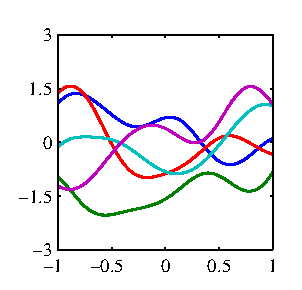
\includegraphics[clip, width=3cm]{charts/Figure6_4a.eps}
  \hspace{1cm}
  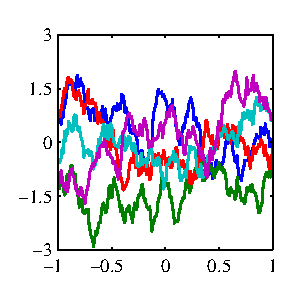
\includegraphics[clip, width=3cm]{charts/Figure6_4b.eps}

  左:
  $k(\mathbf{x}, \mathbf{x'}) = 
  \exp( - \|\mathbf{x} - \mathbf{x'}\|^2 / 2\sigma^2)
  $ {\optima (6.23)}

  右:
  $k(x, x') = \exp( - \theta |x - x'|)$ {\optima (6.56)} 

  \vspace{0.6cm}
  {\optima(6.56)}は、もともとは\textbf{オルンシュタインーウーレンベック過程}
  {\optima(Ornstein-Uhlenbeck process)}というブラウン運動を記述するために
  作られたモデル。

  %  \begin{figure}[htbp]
  %\begin{center}
  %  \begin{tabular}{c}

  %    % 1
  %    \begin{minipage}{0.33\hsize}
  %      \begin{center}
  %        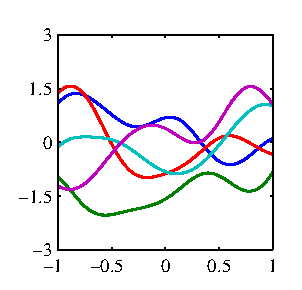
\includegraphics[clip, width=4.5cm]{charts/Figure6_4a.eps}
  %        \hspace{1.6cm} [1]
  %        $k(\mathbf{x}, \mathbf{x'}) = 
  %        \exp( - \|\mathbf{x} - \mathbf{x'}\|^2 / 2\sigma^2)
  %        $ {\optima (6.23)}
  %      \end{center}
  %    \end{minipage}

  %    % 2
  %    \begin{minipage}{0.33\hsize}
  %      \begin{center}
  %        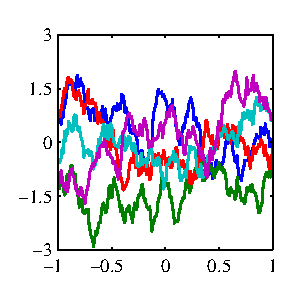
\includegraphics[clip, width=4.5cm]{charts/Figure6_4b.eps}
  %        \hspace{1.6cm} [2]
  %        $k(x, x') = 
  %        \exp( - \theta |x - x'|)
  %        $ {\optima (6.56)}
  %      \end{center}
  %    \end{minipage}

  %\end{tabular}
  %\end{center}
  %\end{figure}
}

% page 8
\frame{
    \frametitle{より一般的には...}
    ガウス過程とは、$y(\mathbf{x})$がガウス分布に従うような確率過程の
    ことである(つまり、関数の形は必ずしも
    $y(\mathbf{x})=\mathbf{w}^\mathrm{T} {\boldsymbol \phi}(\mathbf{x})$
    でなくてもよい)。\vspace{0.2in}

    入力ベクトルが2次元のときは、特別に\textbf{ガウス確率場}
    {\optima(Gaussian random field)}と呼ばれる。
}

% page 9
\frame{
    \frametitle{6.4.1 まとめ}
    \begin{itemize}
    \item ガウス過程とは、関数の値の集合$\bm{\mathsf{y}}$の同時確率が、
    ガウス分布に従うような確率過程(確率変数の寄せ集め)のこと。
    \item 線形回帰も、パラメータ$\mathbf{w}$がガウス分布に従うとすると、
    各データ点$\mathbf{x}_1, \ldots, \mathbf{x}_N$が与えられた
    時の関数の値$\bm{\mathsf{y}}$もガウス分布に従うので、ガウス過程である。
    \item $y(\mathbf{x})$を
        $y(\mathbf{x}) = \mathbf{w}^\mathrm{T} {\boldsymbol \phi} (\mathbf{x})$
    とすると、
    \begin{align}
    \mathbb{E}[\bm{\mathsf{y}}]
        &= {\boldsymbol \Phi} \mathbb{E}[\mathbf{w}] = \mathbf{0}
    \tag{6.52} \\
    \mathrm{cov}[\bm{\mathsf{y}}]
        &= \mathbb{E}[\bm{\mathsf{yy}}^{\mathrm{T}}]
        = \frac{1}{\alpha} {\boldsymbol \Phi \Phi}^{\mathrm{T}}
        = \mathbf{K} \tag{6.53}% \\
    %\mathbb{E}[y(\mathbf{x}_n) y(\mathbf{x}_m)]
    %    &= k(\mathbf{x}_n, \mathbf{x}_m)
    %\tag{6.55}
    \end{align}
    で表されるような確率過程となる。
    \item カーネル関数をどんなものにするかによって、サンプリングされる関数の
        形も変わってくる。
    \end{itemize}
}
